\section*{Теоретическая часть:}
\begin{enumerate}
    \begin{figure}[h!]
        \noindent\centering{
            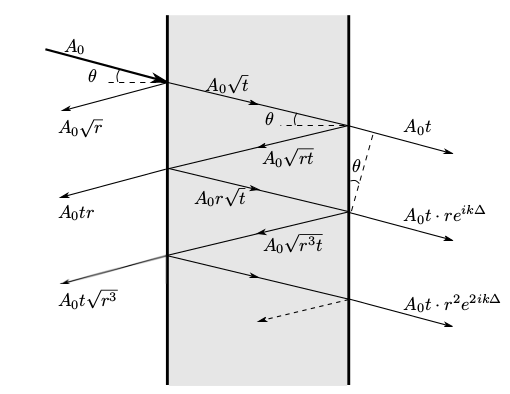
\includegraphics[height = 4cm]{021.png}
        }
        \caption{Амплитуды волн в интерферометре Фабри–Перо. Для прошедших волн также указаны набеги фаз}
    \end{figure}
    \item Разность хода двух интерферирующих волн,
падающих на интерферометр:
\[\Delta = 2L\left( \frac{1}{\cos{\theta}} - \tg{\theta} \sin{\theta} \right) = 2L \cos{\theta}, \]
    где $L$ --- расстояние между зеркалами, или база интерферометра. Интерференционные максимумы:
    \[ 2L \cos{\theta_m} = m \lambda \]
    
    \item Для малых углов $\theta_m \ll 1$ и больших порядков спектра имеем $m \approx M = 2L/\lambda$,
    \[ -2L \sin{\theta_m} d\theta = -2L\theta_m d\theta = m d\lambda \approx \frac{2L}{\lambda}d\lambda, \]
    и угловая дисперсия:
    \[ D = \frac{d\theta}{d\lambda} = -\frac{m}{2L \sin{\theta_m}} \approx -\frac{1}{\lambda\theta_m} \]

    \begin{figure}[h!]
    \centering
    \begin{subfigure}[b]{0.45\textwidth}
        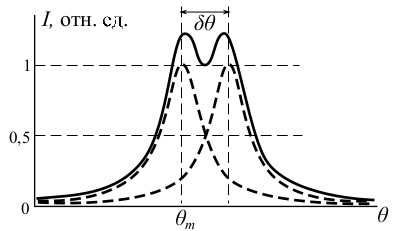
\includegraphics[width=\textwidth]{022.png}
    \end{subfigure}
    \begin{subfigure}[b]{0.45\textwidth}
        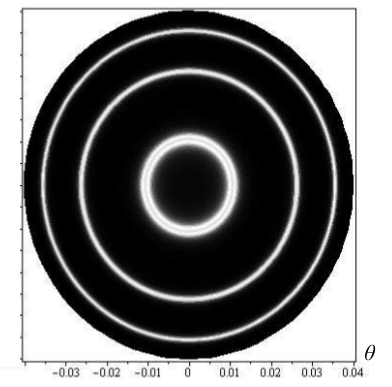
\includegraphics[width=\textwidth]{023.png}
    \end{subfigure}
    \caption{Условие Релея для интерферометра Фабри–Перо: а) интенсивности близких линий и их сумма (схематично); б) расчётное изображение спектра двух близких линий}
    \end{figure}
    \newpage
    Разрешающая способность для порядка спектра $m \approx 2L / \lambda$ равна:
    \[ R = \frac{\lambda}{\delta\lambda} = \frac{\pi\sqrt{r}}{1 - r}m \]
    
\end{enumerate}